\documentclass[12pt]{article}

% Language setting
% Replace `english' with e.g. `spanish' to change the document language
\usepackage[english]{babel}

% Set page size and margins
% Replace `letterpaper' with`a4paper' for UK/EU standard size
\usepackage[letterpaper,top=2cm,bottom=2cm,left=3cm,right=3cm,marginparwidth=1.75cm]{geometry}


%AMS-TeX packages
\usepackage{amssymb,amsmath,amsthm} 
\usepackage{geometry, graphicx}
\usepackage{tabulary}
\usepackage{physics}
\usepackage{enumitem}


% setup the margins
\geometry{margin=1.0in, headheight=15pt}

\usepackage[colorlinks=true, allcolors=blue]{hyperref}
%% Common Declarations %%


\title{PHSX 425, Exam 02}
\author{William Jardee}

\begin{document}
\maketitle

\section*{8.2}
\emph{Consider the charging capacitor in Prob. 7.34}
\begin{figure}[h]
\centering
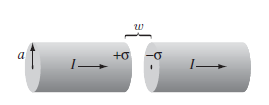
\includegraphics[scale=1]{homework08_question1.png}
\caption{Diagram from question 7.34}
\label{fig:1.1}
\end{figure}
\begin{enumerate}[label=\alph*)]
\item \emph{Find the electric and magnetic fields in the gap, as functions of distance $s$ from the axis and the time $t$. (Assume the charge is zero at $t=0$.)}\bigskip

If we just treat the two surfaces as faces of a parallel plate capacitor:
\[\vb{E}=\frac{\sigma}{\varepsilon_0}\hat{z}\]
where the $\hat{z}$ is pointed the axis of the cylinder to the right. What is $\sigma$? If we consider this the charge that builds up from the current, uniformly distributed over the area:
\[\sigma = \frac{Q}{\pi a^2} = \frac{It}{\pi a^2}\]
Putting this together with the E-field:
\[\boxed{\vb{E} = \frac{It}{\pi a^2 \varepsilon_0}\hat{z}}\]

To find the B-field, we can use $\oint \vb{B} \cdot \dd{\vb{l}} = \mu_0 I_\text{enc} + \mu_0 \varepsilon_0 \int \pdv{\vb{E}}{t}\cdot \dd{\vb{a}}$, recognizing that no current is flowing in the gap.
\[\vb{B}2\pi s = \mu_0 \varepsilon_0 \int \Big(\frac{I}{\pi a^2 \varepsilon_0}\hat{z}\Big)\cdot \dd{\vb{a}}\]
\[B = \frac{\mu_0 I}{2 \pi^2 s a^2} \pi s^2\]
\[\boxed{\vb{B} = \frac{\mu_0 I}{2 \pi a^2} s \, \hat{\phi}}\]

\item \emph{Find the energy density $u_\text{em}$ and the Poynting vector $S$ in the gap. Note especially the direction of $S$. Check that Eq 8.12 is satisfied.}\bigskip

\[u_\text{em} = \frac{1}{2} \varepsilon_0 \vb{E}^2 + \frac{1}{2\mu_0} \vb{B}^2\]
\[= \frac{1}{2} \varepsilon_0 \Big( \frac{It}{\pi a^2 \varepsilon_0} \Big)^2 + \frac{1}{2 \mu_0}\Big( \frac{\mu_0 I}{2 \pi a^2}s\Big)^2\]
\[\boxed{u_\text{em} = \frac{I^2}{2\pi^2 a^4}\Big[ \frac{t^2}{\varepsilon_0} + \frac{\mu_0}{4}s^2\Big]}\]

\[\vb{S} = \frac{1}{\mu_0}\vb{E}\times \vb{B} \]
\[= \frac{1}{\mu_0}\Big(\frac{It}{\pi a^2 \varepsilon_0} \hat{z} \times \frac{\mu_0 I}{2 \pi a^2}s \hat{\phi} \Big) = \boxed{ -\frac{I^2 t s}{2 \pi^2 a^4 \varepsilon_0}\hat{s}}\]

Equation 8.12 states:
\[\pdv{u}{t} = -\div{\vb{S}}\]
Calculating the left hand side first:
\[\pdv{u}{t} = \frac{I^2 t}{\pi^2 a^4 \varepsilon_0}\]
Now for the right hand side:
\[-\div{\vb{S}} = \frac{1}{s}\pdv{s}\frac{I^2 t}{2\pi^2 a^4 \varepsilon_0}s \cdot s = \frac{I^2 t}{\pi^2 a^4 \varepsilon_0}\]
The left and right hand sides both provide the same answer, so equation 8.12 checks out. 

\item \emph{Determine the total energy in the gap, as a function of time. Calculate the total power flowing into the gap, by integrating the Poynting vector over the appropriate surface. Check that the power input is equal to the rate of increase of energy in the gap (Eq. 8.9 - in this case $W=0$, because there is no charge in the gap). [If you're worried about the fringing fields, do it for a volume of radius $b<a$ well inside the gap.]}\bigskip

\[\pdv{U_\textbf{em}}{t} = \int \pdv{u_\text{em}}{t} = -\oint_{\partial V}\vb{S}\cdot \dd{\vb{a}} = \oint_{\partial V}\frac{I^2 t s}{2 \pi^2 a^4 \varepsilon_0} \hat{s} \cdot s \dd{\theta} \dd{z}\hat{s}\eval_{s=a}\]
\[= \frac{I^2 t s^2}{2 \pi^2 a^4 \varepsilon_0}\eval_{s=a} \oint \dd{\theta}\dd{z}\]
\[= \frac{I^2 t}{2 \pi^2 a^ 2 \varepsilon_0} 2\pi w = \boxed{w\frac{I^2 t}{\pi a^2 \varepsilon_0} = \pdv{U_\textbf{em}}{t}}\]

Now, let's follow this up by verifying that this value is correct. 
\[U_\text{em} = \int_V u_\text{em} = \int \frac{I^2}{2\pi^2 a^4}\Big[ \frac{t^2}{\varepsilon_0} + \frac{\mu_0}{4}s^2\Big]s \dd{s} \dd{\theta} \dd{z}\]
\[= w 2\pi \int \frac{I^2}{2\pi^2 a^4}\Big[ \frac{t^2}{\varepsilon_0}s + \frac{\mu_0}{4}s^3\Big] \dd{s}\]
\[= w2\pi \frac{I^2}{2\pi^2 a^4}\Big(\frac{t^2}{\varepsilon_0}\frac{1}{2}s^2 + \frac{\mu_0}{4}\frac{1}{4}s^4\Big)\eval_0^a\]
\[= w \frac{I^2}{2\pi a^4}\Big(\frac{t^2}{\varepsilon_0}a^2 + \frac{\mu_0}{8}a^4\Big)\]
\[U_\text{em} = w \frac{I^2}{2\pi a^2}\Big(\frac{t^2}{\varepsilon_0} + \frac{\mu_0}{8}a^2\Big)\]

\[\pdv{U_\text{em}}{t} = \pdv{t}\Big(w\frac{I^2}{2 \pi a^2}\Big(\frac{t^2}{\varepsilon_0} + \frac{1}{8}\mu_0 a^2\Big)\Big)\]
\[=w\frac{I^2 2t}{2\pi a^2 \varepsilon_0} = w\frac{I^2 t}{\pi a^2 \varepsilon_0}\]

As we expected, these two methods gave us the same answer! (but we can see that one of them did it a lot faster, and easier)

\end{enumerate}

\section*{Question 2:}
\emph{The tip of a scanning tunneling microscope $(\theta < \alpha$, where $\alpha < \pi/2)$, held at a potential $V_0$, contacts a solid surface $(z=0)$. Assume that the STM tip and the surface it contacts are perfect conductors, but that the point of contact at the origin has resistance $R$. Find the Poynting vector $S$. Then calculate the Poynting flux, $\oint S\cdot \dd{a}$, through a shell of radius $r$ around the resistor.}\bigskip

\[\laplacian{V} =0= \frac{1}{r \sin^2(\theta)}\dv{\theta}\sin(\theta)\dv{\theta}V(\theta)\]
\[\dv{\theta}\sin(\theta)\dv{\theta}V(\theta) = 0\]
\[\sin(\theta)\dv{\theta}V(\theta) = C\]
\[\dv{\theta}V(\theta) = \frac{1}{\sin(\theta)}C\]
\[V(\theta) = C\ln(\abs{\tan(\frac{\theta}{2})}) + V_1\]

We know that at $\theta = \alpha$ that $V(\alpha) = V_0$ and that the potential at the flat surface has to be minimized, since it is a perfect conductor; $V(\frac{\pi}{2}) = 0$
\[V(\frac{\pi}{2}) = C\ln(\tan(\frac{\pi}{4})) + V_1 = 0\]
\[C\ln(1) + V_1 = 0\]
\[V_1 = 0\]

\[V(\alpha) = C \ln(\abs{\tan(\frac{\alpha}{2})}) = V_0\]
\[C = \frac{V_0}{\ln(\abs{\tan(\frac{\alpha}{2})})}\]


\[\vb{E} = -\grad{V}\]
\[= -\frac{1}{r}\pdv{\theta}\Big(C \ln(\abs{\tan(\frac{\theta}{2})})\Big)\]
\[= -\frac{C}{r} \frac{1}{\tan(\frac{\theta}{2})}\sec^2(\frac{\theta}{2})\frac{1}{2}\hat{\theta}\]
\[=-\frac{C}{2r}\frac{\cos(\frac{\theta}{2})}{\cos^2(\frac{\theta}{2})\sin(\frac{\theta}{2})}\hat{\theta}\]
\[=-\frac{C}{2r}\frac{1}{\cos(\frac{\theta}{2})\sin(\frac{\theta}{2})}\hat{\theta}\]
\[= -\frac{C}{r \sin(\theta)}\]
\[\vb{E}= - \frac{V_0}{\ln(\abs{\tan(\frac{\alpha}{2})})}\frac{1}{r \sin(\theta)}\hat{\theta}\]

To find the B-field we can integrate around a loop with radius $s$ where $z>0$. We can recognize that the total current along the cone must be the same at any height, by an argument of symmetry. That current will be whatever can flow through the trip, which by ohms law is: $I_\text{enc} = \frac{V_0}{R}$.

\[\oint \vb{B} \cdot \dd{\vb{l}} = \mu_0 I_\text{enc} + \mu_0 \varepsilon_0 \int \pdv{\vb{E}}{t}\]
\[B 2\pi s = \mu_0 \frac{V_0}{R}\]
\[\vb{B} = \frac{\mu_0 V_0}{Rs}\hat{\phi} = \frac{\mu_0 V_0}{Rr \sin(\theta)}\hat{\phi}\]

\[\vb{S} = \frac{1}{\mu_0} \vb{E} \times \vb{B} = \frac{1}{\mu_0}\frac{\mu_0 V_0^2}{R \ln(\abs{\tan(\frac{\alpha}{2})})}\frac{1}{(r\sin(\theta))^2}\hat{r}\]
\[\boxed{\vb{S} =\frac{V_0^2}{R\ln(\abs{\tan(\frac{\alpha}{2})})}\frac{1}{(r\sin(\theta))^2}\hat{r}}\]

\[\int_{\partial V}\vb{S} \cdot \dd{\vb{a}} = \int_{\theta = \alpha}^{\pi/2} \int_{\phi = 0}^{2\pi} \frac{V_0^2}{R\ln(\abs{\tan(\frac{\alpha}{2})})}\frac{1}{(r\sin(\theta))^2}\hat{r} \cdot r^2 \sin(\theta)\dd{\theta} \dd{\phi}\]
\[=\frac{V_0^2}{R \ln(\abs{\tan(\frac{\alpha}{2})})}2\pi \int_{\theta = \alpha}^{\pi/2} \frac{1}{\sin(\theta)\dd{\theta}}\]
\[= -\frac{V_0^2 2\pi}{R \ln(\abs{\tan(\frac{\alpha}{2})})} \ln(\abs{\tan(\frac{\theta}{2})})\eval_\alpha^{\pi/2}\]
\[\boxed{\int_V \pdv{u_\text{em}}{t} = -\frac{V_0^2 2\pi}{R}}\]

\end{document}